\documentclass[chapter, footnote, a4paper, 10pt]{oblivoir}

\usepackage{fapapersize}  %options: dbl4x6 / newmum / mum
% \usefapapersize{188mm,257mm,25mm,25mm,25mm,30mm}
\usefapapersize{*,*,25mm,25mm,25mm,30mm}

\usepackage{mathtools, amsthm, amssymb}
\usepackage{graphicx, jiwonlipsum}
\graphicspath{{pictures/}}

\usepackage{tabu}
\usepackage{enumitem}

% \linespread{1.4}
\SetHangulspace{1.4}{1.3}

\newtheorem{thm}{정리}[chapter]
\newtheorem{cor}[thm]{보조정리}
\renewcommand{\proofname}{증명}

\DeclareRobustCommand{\myem}[2][\empty]{%
\ifx#1\empty
#2\index{#2}%
\else
#2\index{#2}(#1)\index{#1}%
\fi}

\makeindex
\makepagestyle{myheading}
\makeevenfoot{myheading}{\thepage}{}{}
\makeoddfoot{myheading}{}{}{\thepage}
\makeevenhead{myheading}{2017-1\quad 현대사회의 이해}{}{20170001 홍길동}
\makeoddhead{myheading}{20170001 홍길동}{}{기말고사 대체과제}

% \pagestyle{hangul}
\pagestyle{myheading}

% \setmainhangulfont{HANSolM.ttf}

\begin{document}

\begin{itemize}
\item 첫 번째
\item 두 번째
\item 세 번째
\end{itemize}

\begin{enumerate}
\item 첫 번째
\item 두 번째
\item 세 번째
\end{enumerate}

\noindent
Hello world!

\begin{description}
\item[Stupid BBB] things will not become smart because they are in a list. Things will not become smart because they are in a list.
\item[Smart] things, though, can be presented beautifully in a list.
\end{description}

\tableofcontents*

% !TEX root = Modi_RobustCode.tex
\chapter{균형경기변동이론}

\begin{flushright}
\small\sffamily 이 글은 남상호의 《현대경제변동론》(박영사, 2003)에서 발췌하였다.
\end{flushright}


\section{서론}

앞에서 살펴본 케인지언 경기변동이론의 특징은
경기변동을 시장의 실패 혹은 경제의 불균형 상태로 인하여 발생한
것으로 파악하는데 있었다. 그런데 이들 케인즈학파의 경기변동이론은 1970년대에
발생한 스태그플레이션 현상을 예측하지 못하였을 뿐만 아니라,
사후적인 설명을 제공하는데에도 성공하지 못하였다.
그 중에서 가장 큰 문제점은 (1) 경제상황에 따라 사람들의 예측이
달라질 수 있다는 점과, (2) 경기변동모형의 핵심을 이루는 구조
파라메터의 값을 고정된 것으로 처리하였다는 점이다.

이러한 문제점을 보완하려는 노력의 일환으로 대두된 새로운 이론이
바로 균형경기변동이론\index{균형경기변동이론}(equilibrium business cycle theory\index{equilibrium business cycle theory})이다.
균형경기변동이론은 합리적 기대\index{합리적 기대}(rational expectation\index{rational expectation}),
시장청산\index{시장청산}(market clearing\index{market clearing}), 그리고 개별  경제주체의
최적화 원리\index{최적화 원리}(optimization principle\index{optimization principle})로부터 경기변동 현상이 도출된다고 본다.

개별  경제주체의 최적화 행위란 소비자는 주어진 예산제약하에서
효용을 극대화하고, 기업은 주어진 생산기술제약하에서 이윤을
극대화하는 것을 의미한다. 루카스\index{루카스}(Robert E. Lucas, Jr.\index{Lucas, R.E.})나
사전트\index{사전트}(Thomas J. Sargent\index{Sargent, T.J.}) 등은 예상하지 못한 통화량의 변동이나
외부로부터의 공급충격 등과 같은 교란요인\index{교란요인}이 발생하면 이 교란이
경제의 각 부문으로 전파되면서 개별 경제주체의 최적화 행동으로부터
경기변동이 발생한다고 본다. 결국 사람들이 미래에 대하여 합리적인
기대를 갖고, 미시경제학에 바탕을 둔 개별  경제주체의 최적화
행동원리로부터 경기변동 현상을 설명한다는 점에서 이들의 이론을
균형경기변동이론\index{균형경기변동이론}이라고 부른다.

균형경기변동이론은 경기변동의 발생원인이 무엇인가를 기준으로
화폐적 균형경기변동이론, 실물적 균형경기변동이론, 그리고 무역경기변동이론
등으로 구분된다.
화폐적 경기변동이론\index{화폐적 경기변동이론}은 예상하지 못한 통화충격이 경기변동의 원인이라고 보는 견해이고,
실물적 경기변동이론\index{경기변동이론!실물적}은 생산성 충격이나 석유파동 등과 같은 실물적 요인을
경기변동의 원인이라고 보며, 외국과의 무역으로부터 경기변동이 발생한다고 보는
견해가 무역경기변동이론이다.

다음 절에서는 화폐적 경기변동이론을 살펴보고, 3절에서는
실물적 경기변동이론을, 그리고 4절에서는 기타 경기변동이론을 개관하고자 한다.

\section{화폐적 경기변동이론}

다음과 같은 단순한 총수요--총공급 모형을 이용하여 화폐적 경기변동이론을 살펴보기로 하자:
\begin{align}
(AD) \quad y_t^d &= \beta_1 i_t + \beta_2(m_t - m_{t-1, t}^e) + \epsilon_t
\quad \beta_1, \beta_2 > 0
\\
(AS) \quad  y_t^s &= \gamma_1 i_t + \gamma_2(m_t - m_{t-1, t}^e) + \eta_t
\quad \gamma_1, \gamma_2 > 0
\end{align}
여기서 $i_t$는 $t$기의 이자율, $m_t$\은 $t$기의
통화량(자연대수값), $m_{t-1,t}^e$\은 $t-1$기에 예측한 $t$기의
통화량(자연대수값), 그리고 $\epsilon_t$와 $\eta_t$는 평균이 0이고
서로 독립인 확률적 교란항을 각각 나타낸다.

균형조건($y_t^d=y_t^s$)을 이용하여 위 식을 풀면 내생변수인 $i_t,
y_t$는 예상하지 못한 통화충격인 $m_t - m_{t-1, t}^e$ 및 확률적
교란항인 $\epsilon_t, \eta_t$의 함수로 나타낼 수 있다:
\begin{align}
y_t^* &= f(m_t - m_{t-1, t}^e, \epsilon_t, \eta_t) \\
i_t^* &= g(m_t - m_{t-1, t}^e, \epsilon_t, \eta_t)
\end{align}

결과적으로 예측하지 못한 통화공급량($m_t - m_{t-1, t}^e$)의
변화나, 수요충격\index{수요충격}($\epsilon_t$) 또는
공급충격\index{공급충격}($\eta_t$)이 균형산출량과 균형이자율에
영향을 미치게 된다. 만일 통화당국이
프리드먼\index{프리드먼}(Milton Friedman\index{Friedman, M.})의
권고에 따라 $k$\% 규칙\index{규칙}을 준수한다면 예측하지 못한
통화량의 변화는 발생하지 않으므로 통화충격으로 인한 경기변동은
발생하지 않게 된다. 그러나 현실에서는 통화당국\index{통화당국}이
준칙\index{준칙}에 입각한 통화정책을 수행하지 않거나 또는 민간
경제주체보다 우월한 정보집합을 가지고 있는 경우가 많아서 예측하지
못한 통화공급량의 변화가 존재하게 되고, 이러한 통화충격이 바로
경기변동의 원인이 되기도 한다. 다음으로 수요충격은 소비자 선호의
변화 등을 들 수 있고, 공급충격으로는 1970년대의 석유파동,
1980년대의 노동조합 파업, 1990년 및 2003년의 미국과 이라크간 전쟁
등이 여기에 속한다.

 프리드먼\index{프리드먼}\index{Friedman, M.}을 주축으로 하는
 통화주의자\index{통화주의자}들은 광범위한 실증분석을 바탕으로
 통화량의 급격한 변동이 경제를 불안정하게 만든다고 본다.
 이들이 발견한 주요 실증적 증거는 다음과 같다:
 \begin{enumerate}
 \item[(1)]
 통화공급량의 변화는 경기의 순환주기, 화폐의 유통속도,
 인플레이션 등과 강한 양($+$)의 상관관계\index{상관관계}가 존재한다.
 \item[(2)]
 통화공급량의 변화는 생산량의 변화에 선행(lead)하는 경향이 있다.
 \item[(3)]
 통화량을 주어진 것으로 보면 독립투자, 소비, 생산량 등은 유의적인
 상관관계를 갖지 못한다.
 \end{enumerate}

% 구체적으로 세계 대공황 등은
% 급격한 통화량의 감소에서 비롯된 것이라고 주장한다.

 1970년대에 들어와서 사전트\index{사전트}(T.J. Sargent\index{Sargent, T.J.})와
 노벨상 수상자인 루카스\index{루카스}(R.E. Lucas, Jr.\index{Lucas, R.E.})는 통화주의자\index{통화주의자}들의 주장을 계승\hspace*{0.25em}$\cdot$\hspace*{0.25em}발전시켜
 화폐적 균형경기변동이론을 제시하였다.

 \subsection{총수요--총공급 모형과 화폐적 균형경기변동이론}

경제의 총공급은 총생산함수로부터 구할 수 있으며,
총수요는 소비와 투자의 합으로 얻어진다.
$t$기의 총생산량은 다음과 같이 노동과 자본스톡의 함수로
나타낼 수 있다.
\begin{align}
\begin{split}
Y_t = f(L_t, K_{t-1})Y_t^s &= f\Bigl(\dfrac{P_t}{P_{t-1,t}^e}, i_{t}\Bigr) Y_t^d \\
				&= C\Bigl(\dfrac{P_t}{P_{t-1,t}^e}, i_{t}\Bigr) + I\Bigl(\dfrac{P_t}{P_{t-1,t}^e}, i_{t}\Bigr)
\end{split}
				\end{align}
여기서 ${P_t}/P_{t-1,t}^e$는 실제물가와 기대물가의
비율(상대가격)을, 그리고 $i_t$는 이자율을 각각 나타낸다.

균형조건은 다음과 같다.
 \begin{equation}
 f\Bigl(\dfrac{P_t}{P_{t-1,t}^e}, i_{t}\Bigr)
 = C\Bigl(\dfrac{P_t}{P_{t-1,t}^e}, i_{t}\Bigr) + I\Bigl(\dfrac{P_t}{P_{t-1,t}^e}, i_{t}\Bigr)
  \end{equation}
기대물가가 실제물가와 일치할 때, 즉 $P_{t-1,t}^e=P_t$가 성립할 때,
균형이 성립한다. 이 균형을 우리는 합리적
기대\index{합리적 기대}($P_{t-1,t}^e=P_t$)하의 거시경제균형\index{거시경제균형}이라고 부른다.

$P_{t-1,t}^e=P_t$가 성립하면 균형소득은 일정한 값을 갖지만 그렇지
않을 때에는 균형소득 수준은 변동한다. 구체적으로 $P_{t-1,t}^e<P_t$
또는 $P_{t-1,t}^e>P_t$가 성립하면 균형소득은 진동하게 된다.

화폐수량설\index{화폐수량설}에 의하면 통화량은 물가와 1\,:\,1
대응관계를 가지므로 예기하지 못한 통화량의 변화는 곧 기대물가와
실제물가의 괴리를 초래하게 된다. 예기하지 못한 통화량의 증가가
발생하는 경우, 실제물가 수준은 상승하지만 기대물가 수준은 이전
수준에 그대로 머물러 있게 되어 과소기대현상이 발생한다. 이렇게
되면 총공급이 총수요보다 크게 되어 이자율이 하락하고, 이자율의
하락은 소비와 투자를 증대시켜 총수요곡선을 오른쪽으로 이동시킨다.
한편 이자율의 하락은 자본의 한계생산물을 하락시켜 총공급곡선을
왼쪽으로 이동시킨다. 그런데 총수요곡선의 이동폭보다 총공급곡선의
이동폭이 더 작기 때문에 예측하지 못한 통화량의 증가는 균형소득을
증가시키는 결과를 가져오게 된다.

한편, 예측하지 못한 통화량의 감소는 실제물가와 기대물가간의
괴리($P_{t-1,t}^e>P_t$)를 발생시켜 총수요가 총공급을 초과하게
된다. 따라서 총수요곡선은 왼쪽으로 이동하고, 총공급곡선은
오른쪽으로 이동하여 궁극적으로 균형생산량이 감소하게 된다.


\begin{table}
\setlength\tabulinesep{3pt}
\caption{노동증가율의 변화와 경제변수의 성장경로}\label{tab:tab8-1}
\centering{%
\begin{tabu}{X[2.5]|X|X[2.5]|X}
\tabucline[.5pt]{-}
\rowfont{\sffamily} 경제변수             & 변화방향  &경제변수             & 변화방향   \\ 
\tabucline[.5pt]{-}
근로자당 자본($k$)&             증가 &자본($K$)&               불분명\\
근로자당 자본증가율(${\hat k}$)&불변 &자본증가율(${\hat K}$)   & 감소\\
근로자당 소득($y$)&             증가 &이자율($r$)&               하락\\
근로자당 소득증가율(${\hat y}$)&불변 &임금($w$)&                 증가\\
자본계수($v$)&             증가 &소득분배 비율($rK/wL$)&  불분명\\
국민소득($Y$)&           불분명 &근로자당  소비($C/L$)&        증가\\
국민소득증가율(${\hat Y}$)&감소 &                            &   \\
\tabucline[.5pt]{-}
\end{tabu}
}
\end{table}


% !TEX root = Modi_RobustCode.tex
\chapter{여러 가지 곡면}


함수의 연속성이나 미분가능성은 각각의 점에서 정의하기 때문에 \myem{국소적 개념}이라고 말한다. 
하지만 이를 이용하여 주어진 함수의 정의역 전체에서 연속성이나 미분가능성을 정의하므로 함수의 대역적 성질에 대해서도 이야기 할 수 있다. 같은 이유에 의해 가우스곡률과 평균곡률도 국소적 개념이라고 할 수 있지만 이러한 기하학적 개념이 곡면의 국소적 성질이나 모양에만 영향을 미치는 것만은 아니다. 
예를 들어, 주어진 곡면의 모든 점에서 가우스곡률이 $0$이면 이 곡면은 평면이 된다. \myem{가우스곡률}이 모든 점에서 $0$이 아닌 상수이면 이 곡면은 구면 또는 구면의 일부가 된다. 이 장에서는 4장에서 배운 내용을 기초로 곡면의 대역적(global)
성질을 살펴보고 여러가지 곡면의 예를 통하여 한 단계 더 심화된
곡면이론에 대하여 알아본다. 1절에서는 곡면의 대역적 성질에 관한 몇 가지 정리를 소개하고 2절에서는 곡면이론에서 매우 중요한 역할을 하는 \myem[surface of revolution]{회전면}에 대하여 다룬다. \myem{회전면}은 한 곡선을 고정된 한 축을 중심으로 회전시켰을 때 얻어지는
곡면으로 가우스곡률을 비교적 쉽게 구할 수 있다. 또한, 어떤 함수가 주어졌을 때 그 함수를 가우스곡률로 갖는 곡면의
존재성에 관한 문제를 해결해 줄 수 있는 곡면이기도 하다.
3절에서는 곡면의 또다른 예인 \myem[ruled surface]{선직면}에 대하여 알아본다. 선직면은 한 곡선과 그 곡선 위에 정의된
벡터장에 의해 만들어지는 곡면으로 가우스곡률이 항상 $0$보다 작거나 같다. 끝으로 4절에서는
\myem[minimal surfaces]{극소곡면}에 대하여 알아보기로 한다. 극소곡면은 국소적으로 경계를 고정했을 때 넓이가 최소가 되는 곡면이라고 말할 수 있다.



\section{대역적 곡면이론}

이 절에서는 \myem{대역적(global) 곡면이론}에 관한 몇 가지 정리를
소개하고자 한다.
여기서는 주로 \myem{가우스곡률}이 곡면의 위상구조에 어떤 영향을
미치는지에 대하여 알아보기로 한다.  지금까지 그래 왔듯이
앞으로도 \myem{정칙곡면} $M$은 항상 연결집합이라는 것을 가정한다.

\begin{thm}[배꼽점]\label{thm511}
$M \subset \mathbf{R}^3$을 가향 정칙곡면이라 할 때,
가우스함수 $Z$의 미분이 $0$이면, 즉 $\mathrm{d}Z = 0$이면 $M$은 평면
또는 평면의 일부분이다.
\end{thm}

\begin{proof}
한 점 $ \mathbf{p} \in M$을 고정하자. $\mathrm{d}Z = 0$이라는 것은
가우스함수 $Z$가 상수함수임을 나타낸다. 따라서 $M$이
$ \mathbf{p}$를 지나고 $Z$에 수직인 평면에 포함되는 것을
 보이면 된다. $ \mathbf{q}\in M$를 임의의 점이라 하면,
$M$은 연결집합이므로 곡선 $\alpha :[0,1] \to M$이 존재하여
$\alpha(0) =  \mathbf{p}, \alpha(1) =  \mathbf{q}$이다.
이제 함수 $h$를
\[
h(t) = \langle \alpha(t) -  \mathbf{p}, Z \rangle
\]
라 정의하면, $h(0)  =  0$이고 함수 $h$를 $t \in (0,1)$에 대하여 미분하면
\[
h'(t) = \langle \alpha'(t), Z \rangle = 0.
\]
따라서 $h$는 \myem{열린구간} $(0,1)$에서 상수함수이고 $[0,1]$에서 연속함수이므로
닫힌구간 $[0,1]$에서 상수함수이다. $h(0) = 0$이므로 $h(t) = 0$.
특히 $h(1) = \langle  \mathbf{q}-
 \mathbf{p}, Z\rangle = 0$이다. 그러므로 임의의 점
 $ \mathbf{q}\in M$는 우리가 원하는 평면에 놓인다.
\end{proof}

정의에 의해 점 $ \mathbf{p}\in M$가 평면점이면
$\kappa_1( \mathbf{p}) = \kappa_2( \mathbf{p}) = 0$이다. 그리고
이것은 $\mathrm{d}Z_{ \mathbf{p}} = 0$인 것과 동치이다.
정리 \ref{thm511}은 정칙곡면 $M$의 모든 점이 평면점이면 $M$은 평면이라는 것을
보여준다.

\myem{법곡률}의 최대값과 최소값이 일치하는 점을 \myem{배꼽점}이라 말한다. 예를 들어
평면이나 구면의 모든 점은 \myem{배꼽점}이다 (4장1절 참고).
중요한 것은 그것의 역 또한 성립한다는 사실이다.

\begin{thm}\label{thm512}
$M \subset \mathbf{R}^3$을 연결 정칙곡면이라 하자. 만일 $M$의
모든 점이 배꼽점이면 $M$은 구면이나 평면, 또는 그것의 일부분이다.
\end{thm}

\begin{proof}
\textbf{첫째단계:} 점 $\mathbf{p} \in M$가 배꼽점이면 모든 접벡터
$\mathbf{v}\in T_{\mathbf{p}}$는 \myem{주곡률 방향}임을 보이자.

$\mathbf{p}\in M$에서
$\kappa_1(\mathbf{p}) = \kappa_2(\mathbf{p}) = k$이고 $\mathbf{e}_1, \mathbf{e}_2$를
주곡률 방향이라고 하자. 그러면 임의의 접벡터 $\mathbf{v} = a \mathbf{e}_1 +
b \mathbf{e}_2 \in T_{\mathbf{p}} M$에 대하여
\begin{align}
\mathrm{d}Z_{\mathbf{p}}(\mathbf{v})
&= a\, \mathrm{d}Z_{\mathbf{p}}(\mathbf{e}_1) +
b \,\mathrm{d}Z_{\mathbf{p}}(\mathbf{e}_2)\\
&= -a \,k\,  \mathbf{e}_1 - b\, k\,\mathbf{e}_2\\
&= -k \,\mathbf{v}.
\end{align}

\textbf{둘째단계:} $\mathbf{x}: D \subset \mathbf{R}^2 \to M$을 좌표함수라 하고 $V = \mathbf{x}(D)$라
놓자. 그러면 $V$는 평면 또는 구면의 일부분임을 증명하자.

가정에 의해 각 점 $\mathbf{q}\in V$가 배꼽점이므로 \textbf{첫단계}에 의해
임의의 접벡터 $\mathbf{v} = a \mathbf{x}_u + b \mathbf{x}_v \in
T_{\mathbf{q}} M$에 대하여
\begin{equation}
\mathrm{d}Z_{\mathbf{q}}(\mathbf{v}) = \lambda(\mathbf{q}) \mathbf{v}.
\label{eqn21010}
\end{equation}
여기서 $\lambda(\mathbf{q}) = - \kappa_1(\mathbf{q}) = -\kappa_2(\mathbf{q})$는 $V$에서
정의된 미분가능한 함수이다.

\begin{itemize}
\item[\textbf{(i)}] $\lambda$는 \myem{상수함수}이다.
식 \eqref{eqn21010}\를 풀어쓰고 도움정리를 이용하면
\begin{align}
&a dZ(\mathbf{x}_u) + b dZ(\mathbf{x}_v) = \lambda (a \mathbf{x}_u + b \mathbf{x}_v)\\
\Leftrightarrow{}& a Z_u + b Z_v = \lambda (a \mathbf{x}_u + b \mathbf{x}_v).
\end{align}
$\mathbf{v}$는 임의의 \myem{접벡터}이므로
\[
Z_u = \lambda \mathbf{x}_u, \qquad Z_v = \lambda \mathbf{x}_v.
\]
첫째 식을 $v$에 대하여 미분하고 둘째 식을 $u$에 대하여 미분하면
\begin{align}
Z_{uv} &= \lambda_v \mathbf{x}_u + \lambda  \mathbf{x}_{uv}\\
Z_{v u} &= \lambda_u \mathbf{x}_v + \lambda  \mathbf{x}_{vu}.
\end{align}
이 두 식의 뺄셈을 하면
\[
\lambda_v \mathbf{x}_u - \lambda_u  \mathbf{x}_v =0
\]
을 얻는다. $\mathbf{x}_u$와 $\mathbf{x}_v$는 각각의 접평면에서
일차독립이므로 각 점 $\mathbf{q}\in V$에 대하여
\[
\lambda_u = \lambda_v = 0
\]
을 만족한다. $V$연결집합이므로 다변수해석학의 이론에 의해
$\lambda$는 집합 $V$위에서 상수함수이다.

\item[\textbf{(ii)}] $\lambda  = 0$이면 $V$는 평면의 일부이다.

이 경우 $\mathrm{d}Z = 0$이므로 정리 \ref{thm511}에 의해 $V$는 평면 또는 평면의
일부이다.

\item[\textbf{(iii)}] $\lambda \ne 0$이면 $V$는 구면의 일부이다.

다음 벡터방정식
\begin{equation}
\mathbf{y}(u, v) = \mathbf{x}(u, v) - \frac{1}{\lambda} Z(u, v)\label{eqn21011}
\end{equation}
을 생각하자.
\begin{align}
\mathbf{y}_u &= \mathbf{x}_u - \frac{1}{\lambda} Z_u
= \mathbf{x}_u - \frac{1}{\lambda} \mathrm{d}Z(\mathbf{x}_u)\\
&= \mathbf{x}_u - \frac{1}{\lambda}\left(\lambda \mathbf{x}_u \right) =0.
\end{align}
같은 방법으로
\[
\mathbf{y}_v = 0
\]
임을 보일 수 있다. 따라서 $\mathbf{y} = \mathbf{y}_0$는 상수벡터이다.
그러므로 식 \eqref{eqn21011}에서
\[
\Vert  \mathbf{x} - \mathbf{y}\Vert^2 = \frac{1}{\lambda^2} = \text{상수}
\]
즉, $V = \mathbf{x}(D)$는 반지름이 $\displaystyle{\frac{1}{|\lambda|}}$인
구면의 일부분이다.
\end{itemize}


\begin{figure}
\centering{%
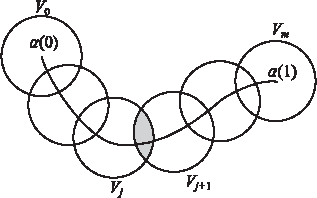
\includegraphics{5-01}
}
\caption{멋진 그림}\label{fig:wonderful_figure}
\end{figure}


\textbf{셋째단계:} $M$ 전체가 평면이나 구면 또는 그것의 일부분임을 증명하자.

둘째 단계에서 좌표함수로 나타낼 수 있는 영역에 대하여 정리가 성립하는 것을
보였다. 셋째 단계에서는 국소적 성질을 대역적 성질로 확장시키는 방법을 이용하여
곡면 전체에 대하여 정리가 성립함을 보이자.

한 점 $\mathbf{p}\in M$을 고정하고 $V\subset M$을
$\mathbf{p}$의 근방으로 하나의 좌표함수로 나태낼 수 있는 영역이라고 하자.
$\mathbf{q}\in M$를 $\mathbf{q}\ne \mathbf{p}$인 임의의 점이라고 하면
연결집합의 정의에 의해
$\alpha(0) = \mathbf{p}$이고 $\alpha(1) = \mathbf{q}$를 만족하는
연속인 곡선 $\alpha : [0,1] \to M$이 존재한다. 각각의 $\alpha(t)$에 대하여
$V_t \subset M$를 하나의 좌표함수로 나타낼 수 있는 $\alpha(t)$의 근방을 택하자.
그러면
\[
\bigcup_{t \in [0,1]}\alpha^{-1}(V_t)
\]
는 닫힌구간 $[0,1]$의 \myem[open covering]{열린덮개}가 된다. $[0,1]$이 \myem{옹골집합}이므로
유한개의 \myem{열린덮개} $\alpha^{-1}(V_1)$, $\cdots$, $\alpha^{-1}(V_m)$, $V_1 = V$가 존재하여
\[
\bigcup_{j= 1}^m\alpha^{-1}(V_j) = [0,1]
\]
이고, 각 $j=1, \cdots, m$에 대하여
\begin{equation}
\alpha^{-1}(V_j) \cap \alpha^{-1}(V_{j+1})\ne \emptyset\label{eqn21012}
\end{equation}
%\vspace{1.5in}
를 만족한다(\figurename~\ref{fig:wonderful_figure}). 따라서
\[
\alpha([0,1]) \subset \bigcup_{j=1}^m V_j.
\]

둘째 단계에 의해 $V_1 = V$는 평면의 일부이거나 구면의 일부이다. 만일 $V_1 = V$가 평면의 일부이면 식 \eqref{eqn21012}에 의해
모든 $j = 1, \cdots, m$에 대하여 $V_j$는 \textbf{같은} 평면의 일부이어야 한다.
따라서 점 $\mathrm{q}$의 근방인 $V_m$도 같은 평면의 일부이다.
만일 $V_1$이 구면의 일부이면 같은 이유에 의해 모든 $j$에 대하여
$V_j$도 같은 구면의 일부이어야만 한다. 결과적으로 $M$ 전체는
평면이거나 구면 또는 그것의 일부분이다.
\end{proof}


정리 \ref{thm512}에 의하면 연결집합인 정칙곡면
 $M$의 모든 점이 배꼽점이면 $M$은 구면 또는 평면이 된다. 따라서
다음 정리가 성립한다.

\begin{cor}\label{cor513}
정칙곡면 $M$의 모든 점이 배꼽점이면 $M$은 상수인 가우스곡률
$K \ge 0$을 갖는다.
\end{cor}

\begin{thm}[정칙곡면과 구의 관계]\label{thm514}
\myem{정칙곡면} $M \subset  \mathbf{R}^3$의 모든 점이 배꼽점이고
$K > 0$이면 $M$은 반지름이 $\displaystyle \frac{1}{\sqrt K}$인 구면 또는
구면의 일부분이다.
\end{thm}

\begin{cor}[당연한 따름정리]\label{surface}
정칙곡면 $M \subset  \mathbf{R}^3$의 모든 점이 \myem{배꼽점}이고
$K > 0$이면 $M$은 반지름이 $\displaystyle \frac{1}{\sqrt K}$인 구면 또는
구면의 일부분이다.
\end{cor}

\begin{proof}[날쌘 정리의 증명]
이 정리는 정리 \ref{thm512}와 따름정리 \ref{cor513}에 의하여 성립한다.
또한 다음과 같은 방법으로 직접 보일 수도  있다.

가정에 의해 각 점 $\mathbf{p}\in M$에서
$\kappa_1(\mathbf{p}) = \kappa_2( \mathbf{p}) = k(\mathbf{p}) \ne 0$이므로
$\kappa(\mathbf{p}) > 0$을 가정해도 된다.
한 점 $\mathbf{p} \in M$을 고정하고 점 $\mathbf{c}$를
\[
\mathbf{c} = \mathbf{p} + \frac{1}{k(\mathbf{p})}
Z(\mathbf{p})
\]
라 놓자. 곡면 위의 임의의 점 $\mathbf{q}\in M$에 대하여 $M$이
연결집합이므로
$\alpha(0) = \mathbf{p}$, $\alpha(1) = \mathbf{q}$인 곡선
$\alpha : [0, 1] \to M$이 존재한다. 이제 곡선 $\gamma$를
\[
\gamma(t) = \alpha(t) + \frac{1}{k(\alpha(t))} Z(\alpha(t)) =
\alpha(t) + \frac 1k Z(t)
\]
라 정의하자. 그러면 도움정리 \ref{cor513}에 의해 $K = k^2$이
상수이므로,
\[
\gamma'(t) = \alpha'(t) + \frac 1k Z'(t)
\]
이다. 한편, $M$의 모든 점이 배꼽점이므로 모든 방향이
주곡률방향이 된다. 따라서
\[
Z'(t) = dZ(\alpha'(t)) = -k \alpha'(t).
\]
그러므로 $\displaystyle \gamma'(t) = \alpha'(t) +
\frac 1k (-k \alpha'(t)) = 0.$
결과적으로
$\gamma$는 상수곡선이 되고, 따라서
\[
\mathbf{c} = \gamma(0) = \gamma(1) = \mathbf{q} +
\frac 1k Z(\mathbf{q}).
\]
다시 말해서, $\displaystyle \Vert \mathbf{q} - \mathbf{c}\Vert = \frac 1k =
\frac{1}{\sqrt K}$이다.
\end{proof}

\begin{proof}
이 정리는 따름정리 \ref{surface}에 의하여 성립한다. 한편, $M$의 모든 점이 배꼽점이므로 모든 방향이
\myem{주곡률 방향}이 된다. 따라서
\[
Z'(t) = dZ(\alpha'(t)) = -k \alpha'(t).
\]
그러므로 $\displaystyle \gamma'(t) = \alpha'(t) +
\frac 1k (-k \alpha'(t)) = 0.$
결과적으로
$\gamma$는 \myem{상수곡선}이 되고, 따라서
\[
\mathbf{c} = \gamma(0) = \gamma(1) = \mathbf{q} +
\frac 1k Z(\mathbf{q}).
\]
\end{proof}

\begin{proof}
$M$의 모든 점이 배꼽점이므로 모든 방향이
\myem{주곡률 방향}이 된다. 따라서
\[
Z'(t) = dZ(\alpha'(t)) = -k \alpha'(t).
\]
그러므로 $\displaystyle \gamma'(t) = \alpha'(t) +
\frac 1k (-k \alpha'(t)) = 0.$
결과적으로
$\gamma$는 \myem{상수곡선}이 되고, 따라서
\[
\mathbf{c} = \gamma(0) = \gamma(1) = \mathbf{q} +
\frac 1k Z(\mathbf{q}).\qedhere
\]
\end{proof}

% !TEX root = Modi_RobustCode.tex

\chapter[일야구도하기]{일야구도하기(一夜九渡河記)}

\begin{flushright}
\small\sffamily 이 글은 박지원의 《열하일기》(1780년 6월부터 2개월간 겪은 일) 중 발췌하였다.\\ jiwonlipsum 패키지를 이용한다.
\end{flushright}

\section{한글 번역}
\jiwon[1-12]

\section{한글에 한자 병기}
\jiwon[13-20]

\section{원문}
\jiwon[21-28]

\section{두보의 絶句}
江碧鳥逾白 \quad  강이 푸르니 새 더욱 희고\\
강벽조유백 \\
山靑花欲然 \quad 산이 푸르니 꽃 빛이 불 붙는듯하다.\\
산청화욕연 \\
今春看又過 \quad 올봄이 또 지나가니\\
금춘간우과  \\
何日是歸年 \quad 어느 날이 이 돌아갈 해오.\\
하일시귀년 



\section{I talk to the wind}
\linespread{1.2}\selectfont
{\raggedleft King Crimson\par}
\begin{center}
Said the straight man to the late man\\
``Where have you been?''\\
I've been here and I've been there\\
And I've been in between
\medskip

(repeat) I talk to the wind\\
My words are all carried away\\
I talk to the wind\\
The wind does not hear, the wind cannot hear
\medskip

I'm on the outside looking inside\\
What do I see\\
Much confusion, disillusion\\
All around me
\medskip

I talk to the wind\\
My words are all carried away\\
I talk to the wind\\
The wind does not hear, the wind cannot hear
\medskip

You don't possess me don't impress me\\
Just upset my mind\\
Can't instruct me or conduct me\\
Just use up my time
\medskip

I talk to the wind\\
My words are all carried away\\
I talk to the wind\\
The wind does not hear, the wind cannot hear
\medskip

I talk to the wind\\
My words are all carried away\\
I talk to the wind\\
The wind does not hear, the wind cannot hear
\end{center}

\linespread{1.4}\selectfont
% !TEX root = Modi_RobustCode.tex

\chapter[S자 이야기]{S자 이야기(Letter S)}


\begin{flushright}
\small\sffamily 이 글은 도널드 크누스가 쓴 \emph{Digital Typography}(CSLI, 1999)에서 발췌하였다. 
\end{flushright}


\noindent 도널드 크누스(Donald E. Knuth) 교수가 쓴
    \href{http://www-cs-faculty.stanford.edu/~knuth/dt.html}{\emph{Digital Typography}}에
    재미있는 꼭지가 있습니다. ``S자 이야기(The Letter S)''인데요,
    프란체스코 토르니엘로(Francesco Torniello)라는 이탈리아의 한
    타이포그래퍼가 쓴 알파벳 도해법에서 S자 도해를 수학적으로 계산하여
    설명하고 있습니다. 재미있는 부분이라는 생각이 들어서 조금
    인용해봅니다. 원문 그대로 옮기지는 않았고요, 제가 중간중간에
    이해를 돕기 위해 추가한 부분이 있습니다만 따로 명기하지는
    않았습니다. 


\section{S자 이야기 중}
 
몇 년 전 최신 프린트 장비에 사용할 적당한 알파벳을 디자인해야하는
문제가 있었는데 문자 스물다섯 개는 비교적 다루기가 쉬웠다. 그렇지 않은
다른 하나는 바로 `S'자였다.
\medskip

(중략)
\bigskip
\begin{figure}
\centering{%

\includegraphics[width=.35\textwidth]{pictures/LAlfabeto}\qquad

\includegraphics[width=.35\textwidth]{pictures/DigitalTypography}
\caption{프란체스코 토르니엘로, 《알파베토》, 1517(왼쪽)와 도널드 크누스, 《디지털 타이포그래피》, 1999}\label{fig:books}}
\end{figure}


프란체스코 토르니엘로가 1517년에 쓴
《알파베토》({\small \textit{L'Alfabeto}})라는 책에는 알파벳 작도법이 소개되어 있다. 
이 가운데 `S'자 작도법을 요즘 수학 용어로 바꾸면 다음과 같다. 

\begin{quote}
\sffamily
`S'자는 $9 \times 9$ 데카르트 좌표 평면에 그린다. 여기서 $0 \le x \le
9,\ 0 \le y \le 9 $이다. `S'를 그리기 위한 경계점 14개를
정의한다. 편의상 이것들을 $P_1=(x_1, y_1)$, $P_2=(x_2, y_2)$, $\ldots$,
$P_{14}=(x_{14},y_{14})$로 정의한다. 
\end{quote}

\begin{figure}
\centering{%
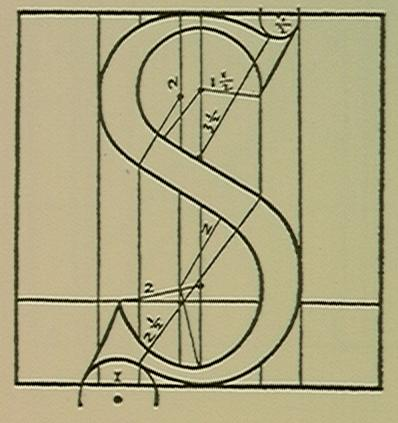
\includegraphics[width=.75\textwidth,height=.80\textwidth,keepaspectratio]{pictures/torniS}
\caption{토르니엘로의 S자 도해}\label{fig:orginal}}
\end{figure}

\begin{enumerate}
\item  중심이 $(4.5, 5.5)$이고 반지름이 $3.5$인 원호를 그린다. 이때
  $P_1$은 원호상의 점 $(4.5, 9)$이다. \label{p:first}


\item 이때 \ref{p:first}에서 그린 원호가 직선 $x=6$와 만나는 점을
  $P_2$라 하자. 그러면 $P_2$는 $(6, 5.5+\sqrt{(3.5)^2 - (1.5)^2})= (6, 5.5+\sqrt{10})$이다.

\item 중심이 $(6.5, 9)$이고 반지름이 $0.5$인 원호를 그릴 차례다. 원호상의
   점 $(6.5, 8.5)$를 $P_3$이라 하고 $P_3$에서 $(7, 9)$까지 원호를 그린다. 

\item 점 $(6, 7)$를 $P_4$이라 하고, $P_4$에서 방금 그린 원호에 접하는
  직선을 긋는다.\label{p:fourth}

\item \ref{p:fourth}에서 원호와 직선의 접점을 $P_5$라 하면  $P_5$는
 $\left (6\frac{16}{17}, 8\frac{13}{17}\right )$이다. (원의 성질과
 닮음비, 삼각비를 이용하여 방정식을 푼다.)


\item 중심이 $(4, 7)$이고 반지름이 $2$인 원호를 그린다. 이때 $P_6$과
  $P_7$은 각각 $(4, 9)$, $(3, 7-\sqrt3)$이다. 이 두 점 사이 만큼
  원호를 그린다.

\item $(5, 4)$를 $P_8$이라 하고 $P_7$에서 $P_8$까지 직선을 긋는다.


\item 중심 $(4.5, 7\frac{1}{8})$에서 $P_4$를 지나는 원호를 $P_9 = (3.5,
  6)$까지 긋는다. 

\item $(6, 4.5)$를 $P_{10}$이라 하고 $P_9$에서 $P_{10}$까지 직선을
  긋는다.

\item $P_{10}$을 지나고 중심이 $(4.5, 2.5)$이고 반지름이 $2.5$인
  반원을 그린다. $P_{11}$은 $(3, 0.5)$이다.

\item $P_{11}$과 $P_{12}$를 잇는  다른 작은 원호를
 그린다. 이 원호의 중심은 $(2.5, y)$이고 반지름은
  $1$인데, $P_{12}$의 $x_{12}$ 좌표는 $1\frac78$이다. 따라서
 $y=(1-\sqrt3)/2 \approx -0.37$이고 $y_{12}=(\sqrt{39}+4-4\sqrt{3}) / 8
 \approx 0.41$이다. (원의 방정식을 풀어야 한다.) 

\item $P_8$에서 (아직 정의되지 않은) $P_{13}$을 잇는 반지름이 $2$인
  원호를 그린다. 이 원호의 중심의 $x$ 좌표는 $4$이고 $x_{13}=
  4.5$이다. 원의 방정식을 풀면 중심은 $(4, 4-\sqrt3) \approx (4,
  2.27)$이고 $y_{13}=4-\sqrt{3}-\sqrt{3.75} \approx 0.33$이다. 

\item $P_{13}$에서 (아직 정의되지 않은) $P_{14}$를 잇는 반지름이 $2$인
  원호를 그린다. 이 원호의 중심의 $y$ 좌표는 $4.5$이고 $y_{14}=
  2$이다. 원의 방정식을 풀면 중심은 $(4.5, 6-\sqrt3-\sqrt{3.75}) \approx (4.5,
  2.33)$이고 $x_{14}=4.5-\sqrt{4-(4-\sqrt{3}-\sqrt{3.75})^2} \approx
  2.53$이다. 

\item 마지막으로 $P_{14}$와 $P_{12}$를 잇는다. 
\end{enumerate}

\bigskip
(인용 끝)


\section{그려보기}

\begin{itemize}

\item 그림~\ref{fig:illustrator}\은 \textsf{Adobe Illustrator}에서
  크누스 교수가 소개한 방법으로 그렸는데, 정확한 작도를 위해 약간의 원의 방정식을 풀어야 했습니다. 

\item 토르니엘로가 그린 다른  문자를 볼 수 있는 곳\\
	\url{http://rubens.anu.edu.au/htdocs/bytype/typefaces/torniello}

\end{itemize}

\begin{figure}
\centering{
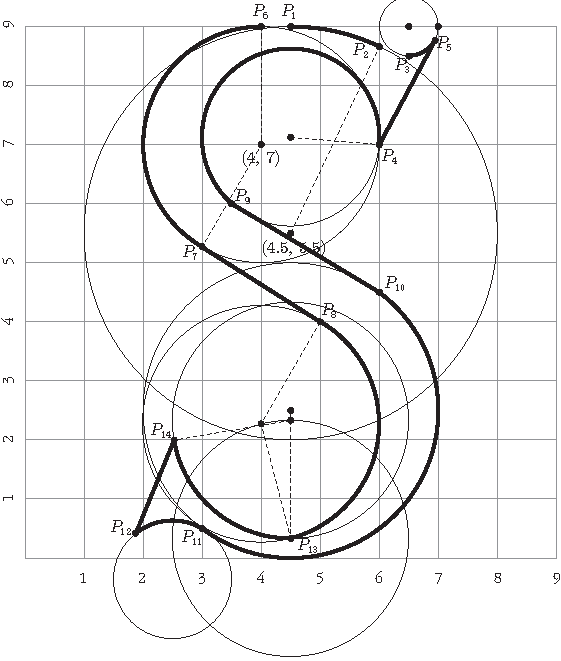
\includegraphics[width=.95\textwidth]{pictures/torniello}
\caption{크누스가 소개한 작도 방법으로 그려본 토르니엘로의 S자}
\label{fig:illustrator}}
\end{figure}

\begin{figure}
\centering{
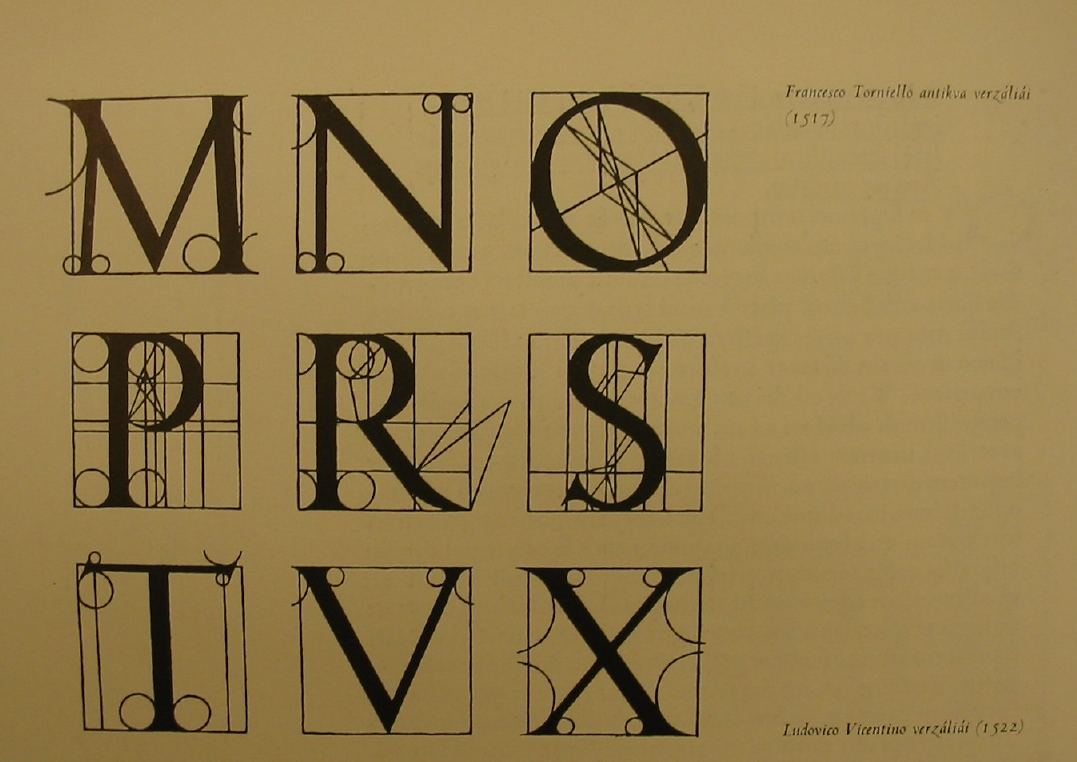
\includegraphics[angle=90, width=.95\textwidth]{pictures/otherletters}
\caption{토르니엘로의 다른 문자}
\label{fig:otherletter}}
\end{figure}


\printindex

\end{document}